% NodeDiffusionTransformer Architecture  (top-to-bottom layout)
% Compile: xelatex node_diffusion_arch.tex
\documentclass[tikz, border=10pt]{standalone}
\usepackage{tikz}
\usepackage{amsmath, amssymb}
\usetikzlibrary{positioning, arrows.meta, fit, backgrounds, calc}

\definecolor{Ccoord}{RGB}{48,118,180}
\definecolor{Ctype}{RGB}{58,145,95}
\definecolor{Ctime}{RGB}{140,95,170}
\definecolor{Ctext}{RGB}{200,128,35}
\definecolor{Cfuse}{RGB}{218,150,38}
\definecolor{Cmodel}{RGB}{65,112,145}
\definecolor{Chead}{RGB}{178,76,66}
\definecolor{Cgray}{RGB}{100,100,100}

\tikzset{
  box/.style={
    draw=#1!58, fill=#1!7, rounded corners=4pt,
    minimum width=2.2cm, minimum height=0.72cm,
    align=center, inner xsep=6pt, inner ysep=4pt,
    font=\scriptsize, line width=0.72pt,
    text=#1!86!black
  },
  wide/.style={
    draw=#1!58, fill=#1!7, rounded corners=4pt,
    minimum width=4.35cm, minimum height=0.78cm,
    align=center, inner xsep=7pt, inner ysep=5pt,
    font=\scriptsize, line width=0.72pt,
    text=#1!86!black
  },
  layer/.style={
    draw=#1!58, fill=#1!6, rounded corners=4pt,
    minimum width=4.10cm, minimum height=0.68cm,
    align=center, inner xsep=6pt, inner ysep=4pt,
    font=\scriptsize, line width=0.72pt,
    text=#1!86!black
  },
  group/.style={
    draw=#1!32, fill=#1!3, rounded corners=6pt,
    line width=0.8pt
  },
  title/.style={
    font=\footnotesize\bfseries, text=#1!82!black
  },
  arr/.style={
    -{Stealth[length=4.8pt,width=3.8pt]},
    line width=0.86pt, color=#1!72
  },
  lightarr/.style={
    -{Stealth[length=4pt,width=3pt]},
    line width=0.68pt, color=#1!58
  }
}

\begin{document}
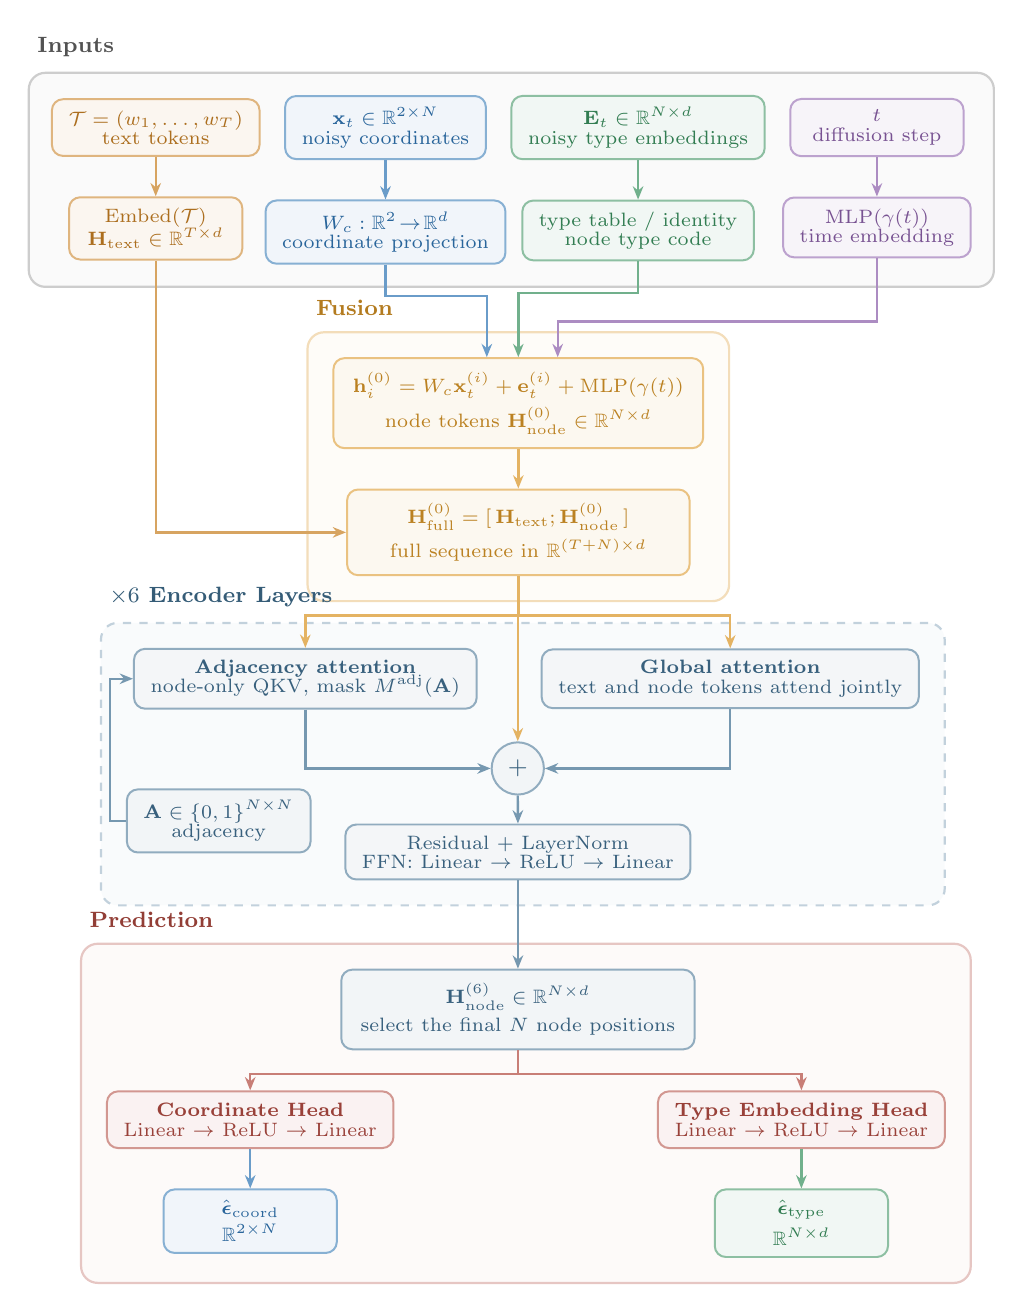
\begin{tikzpicture}[node distance=0.42cm and 0.68cm]

% ---------------------------------------------------------------------
% Row 1: Raw inputs (horizontal)
% ---------------------------------------------------------------------
\node[box=Ctext] at (1.1cm, 0) (txt)
  {$\mathcal{T}=(w_1,\ldots,w_T)$\\[-1pt] text tokens};
\node[box=Ccoord, right=0.3cm of txt] (xin)
  {$\mathbf{x}_t\in\mathbb{R}^{2\times N}$\\[-1pt] noisy coordinates};
\node[box=Ctype, right=0.3cm of xin] (ein)
  {$\mathbf{E}_t\in\mathbb{R}^{N\times d}$\\[-1pt] noisy type embeddings};
\node[box=Ctime, right=0.3cm of ein] (tin)
  {$t$\\[-1pt] diffusion step};

% ---------------------------------------------------------------------
% Row 2: Projections (below each raw input)
% ---------------------------------------------------------------------
\node[box=Ctext, below=0.5cm of txt] (txtemb)
  {$\mathrm{Embed}(\mathcal{T})$\\[-1pt]
   $\mathbf{H}_{\mathrm{text}}\in\mathbb{R}^{T\times d}$};
\node[box=Ccoord, below=0.5cm of xin] (xproj)
  {$W_c:\mathbb{R}^2\!\to\!\mathbb{R}^d$\\[-1pt] coordinate projection};
\node[box=Ctype, below=0.5cm of ein] (eproj)
  {type table / identity\\[-1pt] node type code};
\node[box=Ctime, below=0.5cm of tin] (tproj)
  {$\mathrm{MLP}(\gamma(t))$\\[-1pt] time embedding};

\begin{scope}[on background layer]
  \node[group=Cgray,
        fit=(txt)(xin)(ein)(tin)(txtemb)(xproj)(eproj)(tproj),
        inner sep=8pt] (inputs) {};
\end{scope}
\node[title=Cgray, anchor=south west] at ([yshift=2pt]inputs.north west)
  {Inputs};

% ---------------------------------------------------------------------
% Row 2: Fusion (below inputs, centered)
% ---------------------------------------------------------------------
\node[wide=Cfuse] (nodefuse) at (5.705cm, -3.5cm)
  {$\mathbf{h}^{(0)}_i =
    W_c\mathbf{x}^{(i)}_t+\mathbf{e}^{(i)}_t+\mathrm{MLP}(\gamma(t))$\\[2pt]
   node tokens $\mathbf{H}^{(0)}_{\mathrm{node}}\in\mathbb{R}^{N\times d}$};
\node[wide=Cfuse, below=0.5cm of nodefuse] (seqcat)
  {$\mathbf{H}^{(0)}_{\mathrm{full}}
    =[\,\mathbf{H}_{\mathrm{text}};\mathbf{H}^{(0)}_{\mathrm{node}}\,]$\\[2pt]
   full sequence in $\mathbb{R}^{(T+N)\times d}$};

\begin{scope}[on background layer]
  \node[group=Cfuse, fit=(nodefuse)(seqcat), inner sep=9pt] (fusionbox) {};
\end{scope}
\node[title=Cfuse, anchor=south west] at ([yshift=2pt]fusionbox.north west)
  {Fusion};

% ---------------------------------------------------------------------
% Row 3: Encoder (parallel branches, below fusion)
% ---------------------------------------------------------------------
\node[layer=Cmodel] (adjattn) at (3cm, -7cm)
  {\textbf{Adjacency attention}\\[-1pt]
   node-only QKV, mask $M^{\mathrm{adj}}(\mathbf{A})$};
\node[layer=Cmodel, right=0.8cm of adjattn] (globalattn)
  {\textbf{Global attention}\\[-1pt]
   text and node tokens attend jointly};

\node[circle, draw=Cmodel!58, fill=Cmodel!7, minimum size=0.52cm,
      font=\small, text=Cmodel!86!black, line width=0.72pt]
  (sumnode) at ($(adjattn.south)!0.5!(globalattn.south)+(0,-0.75)$) {$+$};

\node[layer=Cmodel] (ffn) at (5.7cm, -9.2cm)
  {Residual + LayerNorm\\[-1pt]
   FFN: Linear $\to$ ReLU $\to$ Linear};

\node[box=Cmodel, below=1cm of adjattn, xshift=-1.1cm] (adj)
  {$\mathbf{A}\in\{0,1\}^{N\times N}$\\[-1pt] adjacency};

\begin{scope}[on background layer]
  \node[group=Cmodel, dashed,
        fit=(adjattn)(globalattn)(sumnode)(ffn)(adj), inner sep=9pt]
    (encbox) {};
\end{scope}
\node[title=Cmodel, anchor=south west] at ([yshift=2pt]encbox.north west)
  {$\times 6$ Encoder Layers};

% ---------------------------------------------------------------------
% Row 4: Prediction (below encoder)
% ---------------------------------------------------------------------
\node[wide=Cmodel] (nodeout) at (5.7cm, -11.2cm)
  {$\mathbf{H}^{(6)}_{\mathrm{node}}\in\mathbb{R}^{N\times d}$\\[2pt]
   select the final $N$ node positions};

\node[box=Chead] (coordhead) at (2.3cm, -12.6cm)
  {\textbf{Coordinate Head}\\[-1pt] Linear $\to$ ReLU $\to$ Linear};
\node[box=Chead] (typehead) at (9.3cm, -12.6cm)
  {\textbf{Type Embedding Head}\\[-1pt] Linear $\to$ ReLU $\to$ Linear};

\node[box=Ccoord, below=0.5cm of coordhead] (coordout)
  {$\hat{\boldsymbol{\epsilon}}_{\mathrm{coord}}$\\[2pt]
   $\mathbb{R}^{2\times N}$};
\node[box=Ctype, below=0.5cm of typehead] (typeout)
  {$\hat{\boldsymbol{\epsilon}}_{\mathrm{type}}$\\[2pt]
   $\mathbb{R}^{N\times d}$};

\begin{scope}[on background layer]
  \node[group=Chead,
        fit=(nodeout)(coordhead)(typehead)(coordout)(typeout),
        inner sep=9pt] (heads) {};
\end{scope}
\node[title=Chead, anchor=south west] at ([yshift=2pt]heads.north west)
  {Prediction};

% ---------------------------------------------------------------------
% Arrows
% ---------------------------------------------------------------------

% Input row arrows (top → bottom)
\draw[arr=Ctext]  (txt.south)  -- (txtemb.north);
\draw[arr=Ccoord] (xin.south)  -- (xproj.north);
\draw[arr=Ctype]  (ein.south)  -- (eproj.north);
\draw[arr=Ctime]  (tin.south)  -- (tproj.north);

% Inputs → Fusion
\draw[arr=Ctext]  (txtemb.south) |- (seqcat.west);
\draw[arr=Ccoord] (xproj.south)  -- ++(0,-0.4) -| ([xshift=-0.4cm]nodefuse.north);
\draw[arr=Ctype]  (eproj.south)  -- ++(0,-0.4) -| (nodefuse.north);
\draw[arr=Ctime]  (tproj.south)  -- ++(0,-0.8) -| ([xshift=0.5cm]nodefuse.north);

% Fusion internal
\draw[arr=Cfuse] (nodefuse.south) -- (seqcat.north);

% Fusion → Encoder (split to both branches + residual)
\draw[arr=Cfuse] (seqcat.south) -- ++(0,-0.5) -| (adjattn.north);
\draw[arr=Cfuse] (seqcat.south) -- ++(0,-0.5) -| (globalattn.north);
\draw[arr=Cfuse] (seqcat.south) -- ++(0,-0.5) -| (sumnode.north);

% adj → adjattn
\draw[arr=Cmodel] (adj.west) -- ++(-0.2,0) |- (adjattn.west);

% Encoder parallel merge
\draw[arr=Cmodel] (adjattn.south)    |- (sumnode.west);
\draw[arr=Cmodel] (globalattn.south) |- (sumnode.east);
\draw[arr=Cmodel] (sumnode.south)    -- (ffn.north);

% Encoder → Prediction
\draw[arr=Cmodel] (ffn.south) -- (nodeout.north);

% Prediction split
\draw[arr=Chead] (nodeout.south) -- ++(0,-0.3) -| (coordhead.north);
\draw[arr=Chead] (nodeout.south) -- ++(0,-0.3) -| (typehead.north);
\draw[arr=Ccoord] (coordhead.south) -- (coordout.north);
\draw[arr=Ctype]  (typehead.south)  -- (typeout.north);

\end{tikzpicture}
\end{document}
